%!TEX root = ../dokumentation.tex

\chapter{Praktischer Teil: Deployment-Test}
\section{Analyse und Anforderungen}

Der Deployment-Test wurde bereits in Kapitel 3 mehrfach kurz erwähnt. Dieser Test soll unmittelbar nach dem Deployment ablaufen. Die primäre Aufgabe des  %\begin{wrapfigure}{r}{0.45\textwidth}
% \vspace{-30pt}
%  \begin{center}
%   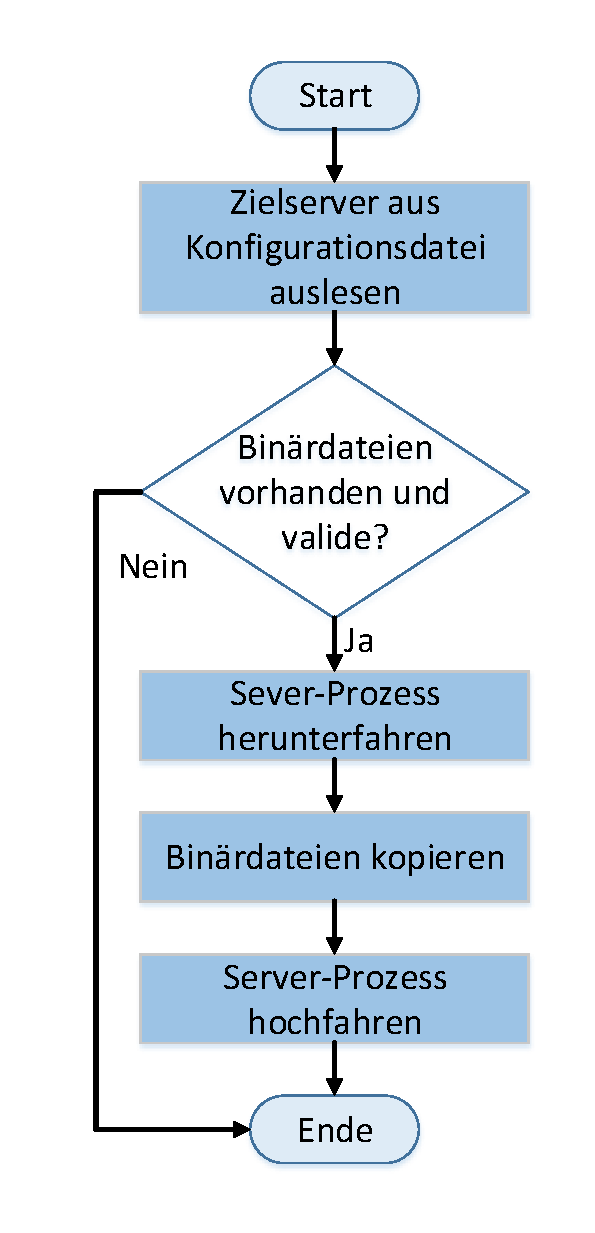
\includegraphics[width=0.45\textwidth]{Deploy_Skript}
%  \end{center}
%\vspace{-35pt}
%  \caption{Ablauf des Deployment Skriptes}
%  \vspace{-20pt}
%  \label{img:Deploy_Pap}
%\end{wrapfigure}
 Deployment-Tests ist es, Fehler während des Deployment Vorganges zu finden und sicherzustellen, dass der Server danach weiterhin fehlerfrei läuft. Da bei der Entwicklung von SAP TwoGo ein Deployment Skript eingesetzt wird, ist es notwendig zu analysieren, welche Schritte dieses Skript abarbeitet. Aus dieser Analyse lassen sich daraufhin die Anforderungen an den Deployment-Test festlegen. Der \acl{PAP} in Abbildung \ref{img:Deploy_Pap} zeigt den groben Ablauf des Deployment Skripts. \\
 \begin{figure}[H]
 \centering
 \vspace{-40pt}
 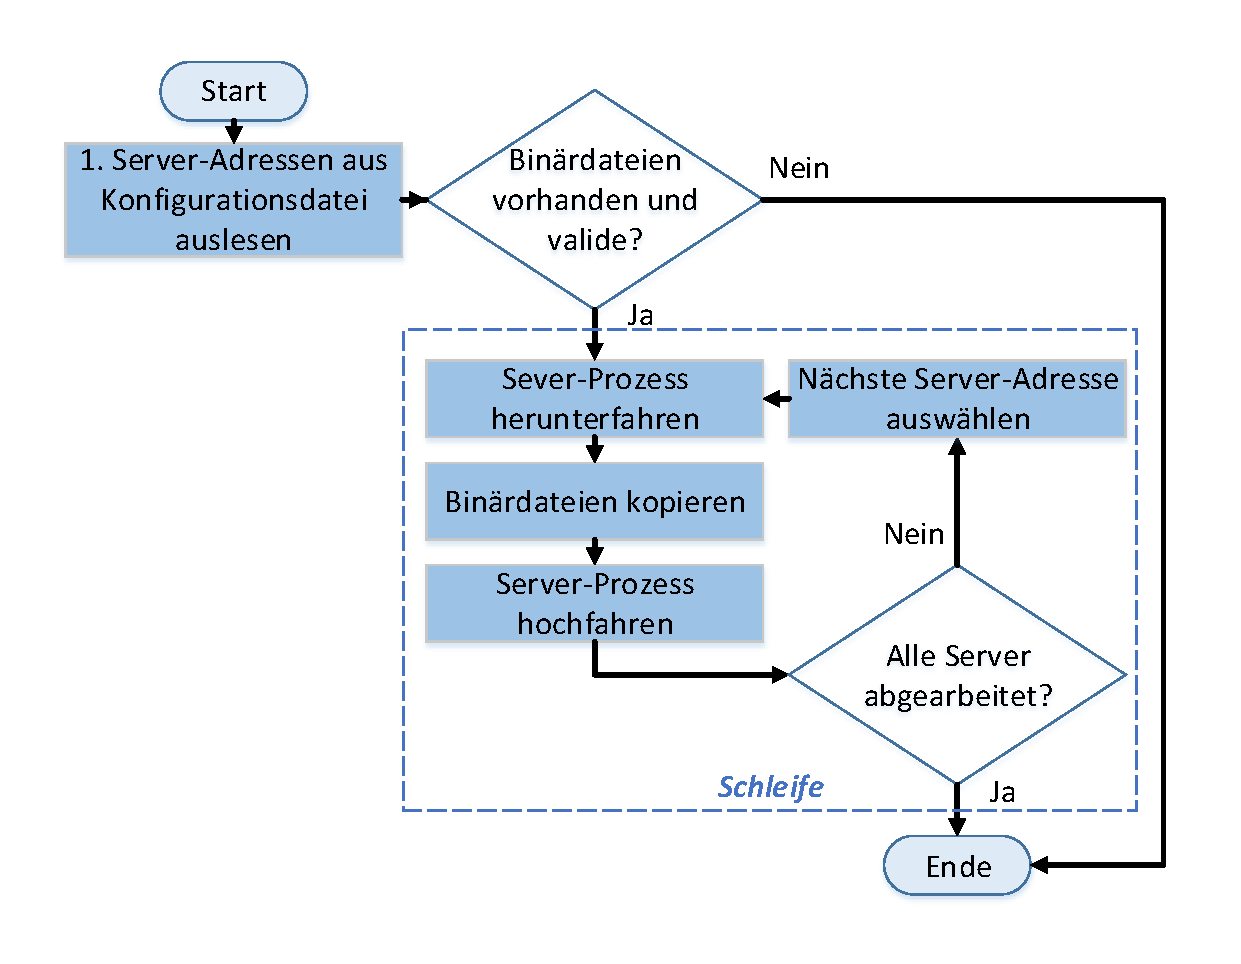
\includegraphics[width=1\linewidth]{../images/Deploy_Skript2.pdf}
 \vspace{-45pt}
 \caption{Ablauf des Deployment Skriptes}
 \vspace{-20pt}
 \label{img:Deploy_Pap}
 \end{figure}
 
Zunächst liest das Skript bei Start eine \textit{.landscape} Konfigurationsdatei. Diese enthält alle Serveradressen einer einzelnen Landschaft, wie zum Beispiel die Adressen des Datenbankservers, Backend-Servers und Matchfinder-Servers der Produktivlandschaft. Im nächsten Schritt wird überprüft, ob die Binärdateien vorhanden sind. Danach werden diese temporär entpackt. Damit wird sichergestellt, dass keine Dateifehler vorhanden sind und das Entpacken später fehlerfrei abläuft. Nach diesen Sicherungsschritten beginnt das eigentliche Deployment. Mithilfe einer Schleife werden die einzelnen Server der gewählten Landschaft nacheinander abgearbeitet. In der Schleife wird zunächst der Server-Prozess heruntergefahren, damit  im Anschluss daran die Binärdateien kopiert werden können. Im letzten Schritt der Schleife wird der Server-Prozess wieder hochgefahren. Während des Hochfahrens wird eine Log-Datei erstellt. In dieser ist unter anderem gespeichert, ob alle Teilsysteme von TwoGo, wie die Oberfläche oder das Administrationstool, korrekt gestartet worden sind und welchen Inhalt bestimmte Umgebungsvariablen haben. Abbildung \ref{fig:Log_part} zeigt einen Ausschnitt der Log-Datei.\\
\begin{figure}[H]
\centering
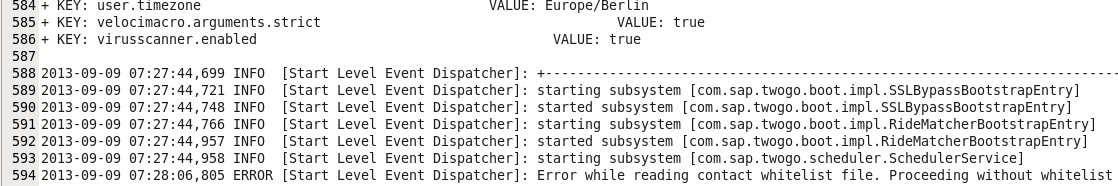
\includegraphics[width=1\linewidth]{../images/Log_part}
\vspace{-20pt}
\caption{Ausschnitt aus Log-Datei}
\label{fig:Log_part}
\end{figure}
 Nach dem Hochfahren wird überprüft, ob alle Server der Konfigurationsdatei abgearbeitet worden sind. Falls dies noch nicht zutrifft, werden die gleichen Schritte für den nächsten Server durchgeführt. Ansonsten wird das Deployment Skript beendet. \\
Anhand dieser Analyse lässt sich erkennen, an welchen Stellen Fehler entstehen könnten, die nicht überprüft und gemeldet werden. Zum einen kann das Problem auftreten, dass die Server-Prozesse nicht richtig hochgefahren werden. Diese Fehler könnten durch unterschiedliche Parameter verursacht werden. Man müsste somit überprüfen, ob die Server-Prozesse nach dem Hochfahren korrekt laufen. Weiterhin könnten in den Log-Dateien Fehler oder Warnungen protokolliert worden sein. Diese sollten gefunden werden. Beim Hochfahren der Server-Prozesse könnte es ebenfalls dazu kommen, dass die Konnektivität der Server-Prozesse nicht funktioniert oder eingeschränkt ist. Diese sollte ebenfalls überprüft werden.\\
Daraus lassen sich folgende Anforderungen an den Deployment-Test festlegen:
\begin{itemize}
\item Läuft der Server-Prozess?
\item Enthält die Log-Datei Fehler?
\item Enthält die Log-Datei Warnungen?
\item Ist der Server erreichbar?
\end{itemize}

\section{Lösungsansatz}
Durch die Analyse konnte ein Lösungsansatz abgleitet werden. Zunächst stellte sich die Frage, zu welchem Zeitpunkt der Deployment-Test aufgerufen werden soll. Da dieser unmittelbar nach dem Deploymentskript ausgeführt werden soll (vgl. Kapitel 3.2.3), ist es logisch, den Test am Ende des Skriptes automatisch aufzurufen. Der Erfolg des Deployment-Tests, und damit verbunden des gesamten Deployments, kann über eine neue Log-Datei ermittelt werden, welche das Resultat jeder einzelnen Überprüfung enthält. Diese Überprüfungen entsprechen den Anforderungen aus Kapitel 4.1. Ihre Abarbeitung wird in dem \acs{PAP} in Abbildung \ref{fig:Deploy_Test} dargestellt.
\begin{figure}[H]
\centering
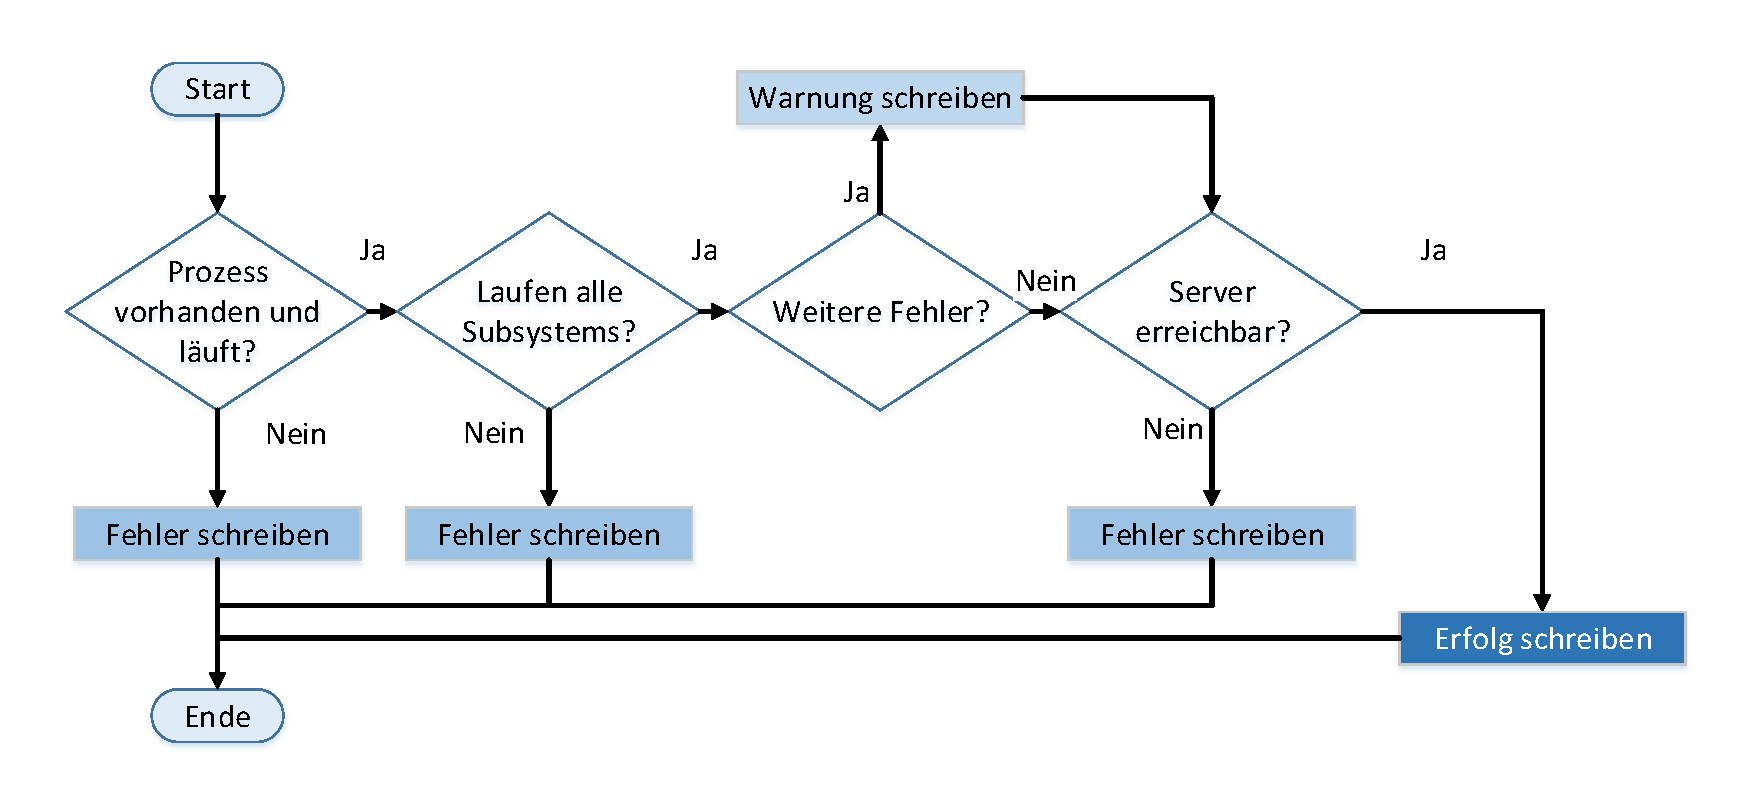
\includegraphics[width=1\linewidth]{../images/Deploy_Test}
\vspace{-50pt}
\caption{Ablauf des Deployment Tests}
\vspace{-5pt}
\label{fig:Deploy_Test}
\end{figure}

\begin{enumerate}
\item \textit{Läuft der Server-Prozess?}
Da der Server-Prozess eine notwendige Voraussetzung für den Betrieb von TwoGo ist, wird im ersten Schritt geprüft, ob dieser Prozess läuft. Sollte dies nicht der Fall sein ist es nicht mehr nötig, die folgenden Schritte auszuführen und der Test kann beendet werden.
\item \textit{Enthält die Log-Datei Fehler?}
Um Fehler innerhalb der Log-Datei zu entdecken, muss diese zunächst einmal existieren. Trifft dies zu, muss der Deployment-Test sechs mal die Zeile \textit{started subsystem} finden. Dieser Wert ergibt sich aus der Anzahl der Komponenten von TwoGo. Sollten nicht alle Systeme laufen, kann der Test ebenfalls abgebrochen werden, da TwoGo sonst nicht fehlerfrei funktionieren kann.
\item \textit{Enthält die Log-Datei Warnungen?}
Zwischen den Meldungen \textit{started subsystem} könnten weitere Fehler auftreten, die Punkt 2 nicht entdeckt. Dazu wird überprüft, ob alle Meldungen innerhalb von 14 Zeilen vorhanden sind. Dieser Wert wurde durch Versuche ermittelt, deren Ergebnis war, dass alle Fehlermeldungen wesentlich länger als 14 Zeilen sind. Da diese Fehler nicht zwangsläufig den Betrieb von TwoGo stören, wird nur eine Warnung gespeichert und darauf hingewiesen, dass die Log-Datei des Prozesses manuell überprüft werden sollte.
\item \textit{Ist der Server erreichbar?}
Die letzte Überprüfung soll gewährleisten, dass der Server auch von außerhalb erreichbar ist. Um dies zuverlässig sicherzustellen, wird ein \acs{JSON} Objekt an den Server gesendet. Dieser \acs{JSON}-\acs{RPC} ist Bestandteil der TwoGo \acs{API}. Sollte das \acs{JSON} Objekt nicht ankommen oder die falsche Antwort vom Server zurückkommen wird eine Fehlermeldung generiert.
\end{enumerate}
Nach dem Durchlauf des Deployment-Tests wird dem Nutzer, der das Deployment Skript gestartet hat, die aus diesen Überprüfungen entstandene Log-Datei angezeigt.
%Die aus diesen Überprüfungen entstandene Log-Datei wird, nach dem Durchlauf des Deployment Tests, dem Nutzer angezeigt der das Deploymentskript gestartet hat.


\section{Implementierung}
Damit der Deployment-Test einfach und effektiv im Deployment Skript aufgerufen werden kann, sollte der Test in der selben Sprache geschrieben werden wie das Deployment  Skript. Dieses ist ein Shell Skript und ist in \acs{Bash} geschrieben. Somit ist die Frage, mit welcher Technologie das Skript realisiert wird, bereits beantwortet. Durch die Verwendung von \acs{Bash} wird außerdem ein einfacher Zugriff auf Betriebssystem-Befehle und Dateiverwaltung gewährleistet.\\
Um den \acs{PAP} in Abbildung \ref{fig:Deploy_Test} am einfachsten zu implementieren, wurden die vier Überprüfungen mithilfe von Funktionen realisiert. Durch diesen Schritt wird das Skript sehr übersichtlich und es entstehen drei Bereiche. Im ersten Teil werden Variablen deklariert, welche beispielsweise Dateipfade enthalten. Die Funktionen sind im zweiten Teil gespeichert und im dritten Teil ist das eigentliche Hauptprogramm, welches die Funktionen aufruft und die Log-Datei schreibt. Die Reihenfolge dieser Teile sind bei \acs{Bash} notwendig, um die Funktionalität zu gewährleisten. Dies beruht darauf, dass die Funktionen die Variablen nutzen und vom Hauptprogramm aufgerufen werden. Diese Teilung ermöglicht es außerdem, spätere Änderungen leicht vorzunehmen. Daraus ergibt sich folgendes Hauptprogramm:
\begin{lstlisting}
check_PID $#     
	if [ $? -eq 1 ]; then
	echo "11||Process is running" >> $dLog_file
	else
	echo "00||Process is NOT running" >> $dLog_file
	exit 0
	fi
check_log $*     
	if [ $? -eq 1 ]; then
	echo "11||Logfile is ok" >> $dLog_file
	else
	echo "00||Not all subsystems have been started" >> $dLog_file
	exit 0
	fi
check_warning $*
	if [ $? -eq 1 ]; then
	echo "11||No warnings" >> $dLog_file
	else 
	echo "10||Please check the log manually" >> $dLog_file
	fi
check_JSON $*
	if [ $? -eq 1 ]; then
	echo "11||Connected to server" >> $dLog_file
	else
	echo "00||Problem with server connection" >> $dLog_file
	fi

\end{lstlisting}

Der Aufruf des Deployment-Tests wird, wie bereits erwähnt, vom Deployment Skript ausgeführt. Um zu erreichen, dass der Test auch auf den jeweiligen Servern läuft, wird er über den Befehl \textit{ssh} aufgerufen. Um zu gewährleisten, dass der Anwender, der das Skript aufruft, auch direkt die Fehlermeldungen aus dem Log des Deployment-Test erhält, werden diese im Deployment Skript ausgelesen. Dazu wird eine Schleife benutzt, welche jede Zeile der Log-Datei liest, herausfindet um welche Art von Fehler es sich handelt und die entsprechende Nachricht schreibt.
\begin{lstlisting}
while read line 
  do 
		   if [[ $line == *00* ]] ; then		# 00 == Error
		      text=${line#*||}
		      writeError "$text"			
		   elif [[ $line == *11* ]]; then		# 11 == Info
		      text=${line#*||}
		      writeInfo "$text"	  
		   else 
		      text=${line#*||}
		      writeInfo "$text"				# else == Warning
		   fi
 done < deployCheck.log
\end{lstlisting}

Durch die Integration in das Deployment Skript ist die Implementation der Deployment-Tests abgeschlossen.

\section{Test}
Um die korrekte Funktion des Deployment-Tests sicherzustellen, muss dieser getestet werden. Um dabei nicht auf einen Produktivserver zuzugreifen und somit den Produktivbetrieb zu beeinflussen, wurden alle notwendigen Programme und Konfigurationen auf einer virtuellen Maschine mit Linux als Betriebssystem installiert. Um einen realitätsnahen Test durchzuführen, wurden die aktuellen Binärdateien des Nexus verwendet. Danach wurden diese auf der virtuellen Maschine deployed.\\
Das erste Resultat dieses Tests ergab, dass der Deployment Test bereits gestartet wird, wenn der Server noch hochfährt. Dies führt dazu, dass der Test fehlschlägt. Es war somit notwendig, eine Veränderung vorzunehmen, welche sicherstellt, dass der Deployment-Test erst nach dem Hochfahren ausgeführt wird. Als die einfachste Lösung für dieses Problem hat sich eine Pause herausgestellt. Die Dauer dieser Pause wurde auf Basis mehrerer Testläufe auf 45 Sekunden festgelegt.\\
Ein weiteres Problem ergab sich beim Überprüfen der Konnektivität.  Hier antwortete der Server nicht mit dem erwarteten \acs{JSON} Objekt, sondern mit dem folgenden Objekt:
\begin{figure}[H]
\vspace{-5pt}
\centering
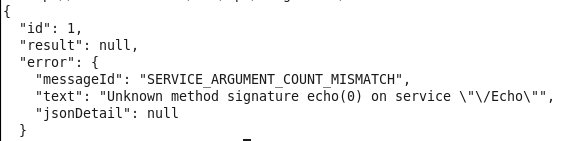
\includegraphics[width=1\textwidth]{../images/json_error}
\vspace{-25pt}
\caption{Falsches JSON Objekt}
\vspace{-10pt}
\label{fig:json_error}
\end{figure}
Der Grund für dieses Verhalten ist, dass bei der Implementation einige Sicherheitsaspekte nicht beachtet wurden. Um ein für den Server gültiges \acs{JSON} Objekt zu senden, muss dieses einen Security-Token und einen Cookie enthalten. Diese können durch das Senden eines anderen \acs{JSON} Objektes  angefordert werden. Danach kann man den Token und das Cookie dem eigentlichen \acs{JSON} Objekt übergeben. Mit dieser Veränderung in der Implementierung des Deplyoment-Tests funktioniert diese Funktion korrekt und das richtige Objekt wird zurückgeliefert:
\begin{figure}[H]
\vspace{-5pt}
\centering
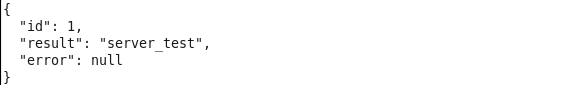
\includegraphics[width=1\textwidth]{json_correct}
\vspace{-25pt}
\caption{Korrektes JSON Objekt}
\vspace{-10pt}
\label{fig:json_correct}
\end{figure}
Neben diesen zwei Fehlern gab es noch weitere kleine Fehler. Diese beruhten jedoch auf Syntaxfehlern und konnten einfach behoben werden. Mit der Überprüfung des Deployment-Tests und der damit verbunden Behebung der Fehler kann sichergestellt werden, dass der Deployment-Test die Anforderungen aus Kapitel 4.1 erfüllt und produktiv eingesetzt werden kann. Damit ist der Deployment-Test vollständig.

